
\documentclass{article}
\usepackage{hyperref}
\usepackage[
    type={CC},
    modifier={by-nc-sa},
    version={3.0},
]{doclicense}
\usepackage[landscape]{geometry}
\usepackage{url}
\usepackage{multicol}
\usepackage{amsmath}
\usepackage{esint}
\usepackage{amsfonts}
\usepackage{tikz}
\usetikzlibrary{decorations.pathmorphing}
\usepackage{amsmath,amssymb}

\usepackage{colortbl}
\usepackage{xcolor}
\usepackage{mathtools}
\usepackage{amsmath,amssymb}
\usepackage{enumitem}
\makeatletter

\newcommand*\bigcdot{\mathpalette\bigcdot@{.5}}
\newcommand*\bigcdot@[2]{\mathbin{\vcenter{\hbox{\scalebox{#2}{$\m@th#1\bullet$}}}}}
\makeatother

\title{PHYS 158 - Making Sense of Circuits}
\usepackage[english]{babel}
\usepackage[utf8]{inputenc}

\renewcommand{\baselinestretch}{1.15}

\advance\topmargin-.8in
\advance\textheight3in
\advance\textwidth3in
\advance\oddsidemargin-1.5in
\advance\evensidemargin-1.5in
\parindent0pt
\parskip2pt
\newcommand{\hr}{\centerline{\rule{3.5in}{1pt}}}
%\colorbox[HTML]{e4e4e4}{\makebox[\textwidth-2\fboxsep][l]{texto}
\begin{document}

\begin{center}{\huge{\textbf{PHYS 158 - Unofficial Formula Sheet}}}\\
\end{center}
\begin{multicols*}{3}

\tikzstyle{mybox} = [draw=black, fill=white, very thick,
    rectangle, rounded corners, inner sep=10pt, inner ysep=10pt]
\tikzstyle{fancytitle} =[fill=black, text=white, font=\bfseries]

 

%------------ Standing Waves ---------------
\begin{tikzpicture}
\node [mybox] (box){%
    \begin{minipage}{0.3\textwidth}
    \textbf{Oscillatory Motion}
    \hline
    \small{
    	\begin{tabular}{lp{4cm} l}
    	\\
		Frequency & $f=\frac{1}{T}$\\
		Angular Frequency & $\omega=2\pi f=\frac{2\pi}{T}$\\
		Wave Number & $k=\frac{2\pi}{\lambda}$\\
		Wave Speed & $v=\lambda f$\\
		Speed of Sound & $v_{sound} \approx 343m/s$\\
		\end{tabular}
	}
	\vspace{.3cm}
	\\
    \textbf{Standing Waves}
    \hline
    \small{
    	\begin{tabular}{lp{5cm} l}
    	\\
		Equation & $y(x,t)=A_{SW}\sin(kx)\sin(\omega t)$\\
		Fundamentals & $f_m=mf_1$
		\vspace{.1cm}\\
		Two End Nodes & $l=\frac{m\lambda}{2}$\\
		One End Node & $l=\frac{m\lambda}{4}$\\
		\end{tabular}

	}
	\vspace{.3cm}
	\\
	\textbf{Beats}
    \hline
    \small{
    	\begin{tabular}{lp{6cm} l}
    	Equation & D(t)=2A\cos(\frac{1}{2}(\omega_1-\omega_2)t)\sin(\frac{1}{2}(\omega_1+\omega_2)t)\\
    	Average Freq & $\frac{1}{2}(f_1+f_2)$\\
    	Beat Freq & $f_{beat}=f_1-f_2=2f_{amp}$
		\end{tabular}
	}
    \end{minipage}
};
%------------ Standing Waves ---------------------
\node[fancytitle, right=10pt] at (box.north west) {Beats and Standing Waves};
\end{tikzpicture}
%------------ Thin Film and Interference ---------------
\begin{tikzpicture}
\node [mybox] (box){%
    \begin{minipage}{0.3\textwidth}
    \textbf{Path Difference}
    \hline
    \small{
    	\begin{tabular}{lp{4cm} l}
    	\\
    	Constructive & $\Delta r = m\lambda_{med}$\\
    	Destructive & $\Delta r = (m-\frac{1}{2})\lambda_{med}$\\
    	Constructive & $\Delta$arg$=2\pi m$\\
    	Destructive & $\Delta$arg$=(2m-1)\pi$\\
		\end{tabular}
	}
	\vspace{.3cm}
	\\
    \textbf{Change of Medium}
    \hline
    \small{
    	\begin{tabular}{lp{4cm} l}
    	\\
    	Speed of Light & $c=2.998\cdot 10^8m/s$\\
    	Index of Refraction & $n=\frac{c}{v_{med}}=\frac{\lambda}{\lambda_{med}}$\\
    	Film Medium Interference & $\Delta r = s_1n_1-n_2s_2$\\
    	Snell's Law & $n_1\sin\theta_1=n_2\sin\theta_2$
		\end{tabular}
	}
	\vspace{.3cm}
	\\
	\textbf{Double Slit}
    \hline
    \small{
    	\begin{tabular}{lp{4cm} l}
    	\\
    	$\Delta r \approx d\sin\theta$ for $d\ll R$\\
    	$\Delta r \approx \frac{dy_m}{R}$ for $d\ll R$ and $d\ll y_m$\\
		\end{tabular}
	}
		\vspace{.3cm}
	\\
	\textbf{Thin Film}
    \hline
    \small{
    	\begin{tabular}{lp{5cm} l}
    	\\
    	Fast to Slow Medium & $\phi = \pi$\\
    	Slow to Fast Medium & $\phi = 0$\\
    	Interference & $\Delta$arg$=2sk_{f}+\Delta \phi=\frac{4s\pi n_{f}}{\lambda}+\Delta \phi$\\
		\end{tabular}
	}
    \end{minipage}
};
%------------ Thin Film and Interference ---------------------
\node[fancytitle, right=10pt] at (box.north west) {Thin Film and Interference};
\end{tikzpicture}

%------------ General Circuits ---------------
\begin{tikzpicture}
\node [mybox] (box){%
    \begin{minipage}{0.3\textwidth}
    \textbf{Resistors}
    \hline
    \small{
    	\begin{tabular}{lp{4cm} l}
    	\\
		Ohm's Law & $V=IR$ \\
		Power Dissipated & $P=V_{ab}I=I^2R=\frac{V_{ab}^2}{R}$\\
		Series & $R_{eq}=R_1 + R_2 + R_3 + ....$\\
		Parallel & $\frac{1}{R_{eq}} = \frac{1}{R_{1}}+\frac{1}{R_{2}}+\frac{1}{R_{3}}+....$\\
		\end{tabular}
	}
	\vspace{.3cm}
	\\
    \textbf{Capacitors}
    \hline
    \small{
    	\begin{tabular}{lp{4cm} l}
    	\\
		Capacitance & $C=\frac{Q}{V_{ab}}$ 
		\vspace{.1cm}\\
		Stored Energy & $U=\frac{Q^2}{2C}=\frac{1}{2}CV^2=\frac{1}{2}QV$
		\vspace{.1cm}\\
		Series &  $\frac{1}{C_{eq}} = \frac{1}{C_{1}}+\frac{1}{C_{2}}+\frac{1}{C_{3}}+....$\\
		Parallel & $C_{eq}=C_1 + C_2 + C_3 + ....$\\
		\end{tabular}

	}
	\vspace{.3cm}
	\\
	\textbf{Inductors}
    \hline
    \small{
    	\begin{tabular}{lp{4cm} l}
    	
		Self-induced emf &$\mathcal{E}_L=-L\frac{di}{dt}$\\
		Power & $dP=i(t)V=iL\frac{di}{dt}$\\
		Stored Energy & $U_L=\frac{1}{2}L\cdot (I_f^2-I_0^2$)\\
		Series & $L_{eq}=L_1 + L_2 + L_3 + ....$\\
		Parallel & $\frac{1}{L_{eq}} = \frac{1}{L_{1}}+\frac{1}{L_{2}}+\frac{1}{L_{3}}+....$\\
		\end{tabular}
	}
    \end{minipage}
};
%------------ General Circuits ---------------------
\node[fancytitle, right=10pt] at (box.north west) {General Circuits};
\end{tikzpicture}

%------------ Time Dependencies RC ---------------
\begin{tikzpicture}
\node [mybox] (box){%
    \begin{minipage}{0.3\textwidth}
    \textbf{RC Circuit Charging}
    \hline
    \vspace{.1cm}\\
    \small{
    1. Find a differential equation to relate the current $i = \frac{dq}{dt}$ \\
    and the charge ($q$) using voltage loop law 
    \\
    \hline
    \vspace{.1cm}\\
    \begin{tabular}{lp{4cm} l}
    	Charging Capacitor & $V-iR-\frac{q}{C}=0$
		\vspace{.1cm}\\
		(derivative) & $-R\frac{di}{dt}-\frac{1}{C}\frac{dq}{dt}=0$
		\vspace{.1cm}\\
		($i=\frac{dq}{dt}$) & $-R\frac{di}{dt}-\frac{1}{C}i=0$
		\vspace{.1cm}\\
		& $\frac{di}{dt} = -\frac{1}{RC}i$
		\vspace{.1cm}\\
		\textbf{Current Function}: & $i(t)=i_0\cdot e^{-\frac{t}{R_{eq}C_{eq}}}$
		\vspace{.1cm}\\
		Substitution & $\frac{dq}{dt}=\frac{V}{R}e^{-\frac{t}{RC}}$
		\vspace{.1cm}\\
		\textbf{Charge Function:} & $q(t)=Q_f(1-e^{-\frac{t}{RC}})$\\
		& $Q_f$= final charge
		\end{tabular}
	}
	\vspace{.2cm}
	\\
	    \textbf{RC Circuit Discharge}
    \hline
    \vspace{.1cm}\\
    \small{

    \begin{tabular}{lp{4cm} l}
    	Discharging Capacitor & $\frac{q(t)}{C}-iR=0$
		\vspace{.1cm}\\
		(rearranging) & $-i=\frac{dq}{dt}=-\frac{1}{RC}\cdot q(t)$
		\vspace{.1cm}\\
		\textbf{Charge Function:} & $q(t)=q_0\cdot e^{-\frac{t}{RC}}$
		\vspace{.1cm}\\
	    ($q_0=CV$)+derivative & $i(t)=i_0e^{-\frac{t}{RC}}$
		\vspace{.1cm}\\
		\textbf{Current Function}: & $i(t)=i_0\cdot e^{-\frac{t}{RC}}$
		\end{tabular}
	}

    \end{minipage}
};
%------------ Time Dependencies RC ---------------------
\node[fancytitle, right=10pt] at (box.north west) {Time Dependent RC};
\end{tikzpicture}

%------------ Time Dependencies RC ---------------
\begin{tikzpicture}
\node [mybox] (box){%
    \begin{minipage}{0.3\textwidth}
    \textbf{RL Circuit Decay}
    \hline
    \vspace{.1cm}\\
    \small{
    1. Find a differential equation to relate the current $i$ and\\
    the change in current $\frac{di}{dt}$ using voltage loop law 
    \\
    \hline
    \vspace{.1cm}\\
    \begin{tabular}{lp{4cm} l}
    	Discharging Inductor & $\mathcal{E}_L-iR=0$
		\vspace{.1cm}\\
		 & $-L\frac{di}{dt}-iR=0$
		\vspace{.1cm}\\
		& $\frac{di}{dt}=-\frac{R}{L}i$
		\vspace{.1cm}\\
		\textbf{Current Function}: & $i(t)=i_0\cdot e^{-\frac{R}{L}t}$
		\end{tabular}
	}
	\vspace{.3cm}
	\\
	    \textbf{RL Circuit Increasing}
        \hline
    \vspace{.1cm}\\
    \small{
    1. Follow the same procedure to solve differential equation\\
    as shown in RC Charging Circuit for Charge Function
    \\
    \hline
    \vspace{.1cm}\\
    \begin{tabular}{lp{4cm} l}
    	Voltage Law & $\mathcal{E}-iR-L\frac{di}{dt}=0$
		\vspace{.1cm}\\
		\textbf{Current Function} & $i(t)=I_{final}(1-e^{-\frac{R}{L}t})$\\
		\end{tabular}
	}

    \end{minipage}
};
%------------ Time Dependencies RL ---------------------
\node[fancytitle, right=10pt] at (box.north west) {Time Dependent RL};
\end{tikzpicture}

%------------ LC Circuits ---------------
\begin{tikzpicture}
\node [mybox] (box){%
    \begin{minipage}{0.3\textwidth}
    \textbf{LC Circuit Oscillations}
    \hline
    \small{
    \vspace{.1cm}\\
    \begin{tabular}{lp{4cm} l}
    	Angular Frequency & $\omega = \sqrt{\frac{1}{LC}}$\\
		Capacitor Charge & $q(t)=Q_{max}\cdot cos(\omega t + \phi)$\\
		$-\frac{dq}{dt}$ (Current) & $i(t)=\omega Q_{max}\cdot sin(\omega t + \phi)$\\
		Energy  & $ \frac{1}{2}Li^2 + \frac{1}{2}\frac{q^2}{C} = \frac{Q_{max}^2}{2C}$
		\vspace{.2cm}\\
		\end{tabular}
	}
    \hline
    \begin{center}
       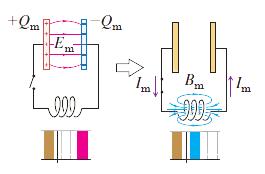
\includegraphics[width=2in]{images/Inductor-removebg-preview.png} 
    \end{center}
    
    \end{minipage}
};
%------------ LC Circuits Header ---------------------
\node[fancytitle, right=10pt] at (box.north west) {LC Circuits};
\end{tikzpicture}

%------------ RLC Circuits ---------------
\begin{tikzpicture}
\node [mybox] (box){%
    \begin{minipage}{0.3\textwidth}
    \textbf{Damped Oscillations}
    \hline
    \small{
    Find the damped $\omega'$similar to LC Circuit but damped \\
    \begin{tabular}{lp{4cm} l}
        Damped Omega & $\omega'=\sqrt{\frac{1}{LC}-\frac{R^2}{4L^2}}$\\
    	Damped Charge & $q(t)=Ae^{-\frac{R}{2L}t}\cdot cos(\omega't+\phi)$\\
		Underdamped if & $\omega' > 0$ 
		\end{tabular}
	}

    
    \end{minipage}
};
%------------ RLC Circuits Header ---------------------
\node[fancytitle, right=10pt] at (box.north west) {RLC Circuits};
\end{tikzpicture}


%-------------------Authorship-----------------------

\begin{center}
    \framebox{
    \parbox[t][.5cm]{7.5cm}{
    \addvspace{0.2cm} \centering 
    \footnotesize Compiled by Simon Ghyselincks and Tyler Wilson 2021 
    } 
}
\end{center}
\end{multicols*}

%------------ CC License -----------------------------
\doclicenseThis

\linespread{1.3}

\begin{multicols*}{3}
\tikzstyle{mybox} = [draw=black, fill=white, very thick,
    rectangle, rounded corners, inner sep=10pt, inner ysep=10pt]
\tikzstyle{fancytitle} =[fill=black, text=white, font=\bfseries]


%--------------New Pages for Electrical --------------------
\newpage
%--------------New Pages for Electrical --------------------


%------------ AC Circuit I and V ---------------
\begin{tikzpicture}
\node [mybox] (box){%
    \begin{minipage}{0.3\textwidth}
    1. Given $V(t) = V_{max}\cdot sin(\omega t+\phi_0)\\$
    2. Solve for I(t) (Note, same phase across L, R, C)
    \vspace{.15cm}\\
    \textbf{Inductive and Capacitive Resistance}\\
    $X_L=\omega L$\\
    $X_C = \frac{1}{\omega C}$
    \vspace{.15cm}\\
    \textbf{Total Impedence Z: }\\
    $\left | Z \right |^2=R^2+(X_L-X_C)^2$
    \vspace{.15cm}\\
    \textbf{Phase Angle:}\\
    $\tan\phi=\frac{X_L-X_C}{R}$\\
    arg$(v)-$arg$(i)=\phi$
    \vspace{.15cm}\\
    \textbf{Current as a function of time:}\\
    $I(t)=\frac{V_{max}}{Z}\cdot sin(\omega t+ \phi_0-\phi)$
    \vspace{.15cm}\\
    \textbf{Individual Voltages:}\\
    $V_R(t) = R\cdot\frac{V_{max}}{Z}\cdot sin(\omega t+ \phi_0-\phi)$\\
    $V_L(t) = X_L\cdot\frac{V_{max}}{Z}\cdot sin(\omega t+ \phi_0-\phi+\frac{\pi}{2})$\\
    $V_C(t) = X_C\cdot\frac{V_{max}}{Z}\cdot sin(\omega t+ \phi_0-\phi-\frac{\pi}{2})$
    \vspace{.15cm}\\
    \textbf{Relation of Max to RMS Voltage:}\\
    $V_{rms}=\frac{1}{\sqrt{2}}\cdot V_{max}$\\
    \textbf{Relation of Max to RMS Current:}\\
    $I_{rms}=\frac{1}{\sqrt{2}}\cdot I_{max}$
    
    
    \end{minipage}
};
%------------ Ac Circuit Header ---------------------
\node[fancytitle, right=10pt] at (box.north west) {AC Series Current and Voltage};
\end{tikzpicture}

%------------ AC Power and Res ---------------
\begin{tikzpicture}
\node [mybox] (box){%
    \begin{minipage}{0.3\textwidth}
    1. Find $\phi$, then $\cos(\phi)$ is the power factor:\\ 
    \textbf{Average Power Function:}\\
    $P_{av}=\frac{1}{2}V_{max}I_{max}\cdot \cos(\phi)=V_{rms}I_{rms}\cdot \cos(\phi)$\\
    $P_{av}=I_{rms}^2R$\\
    $cos(\phi)=\frac{R}{Z}$\\
    \hline
    \vspace{.5 cm}
    For Resonance $X_C=X_L$, peak current and $\phi=0$\\
    \textbf{Resonance}\\
    $\omega_0=\frac{1}{\sqrt{LC}}$
    
    
    
    \end{minipage}
};
%------------ AC Power Header ---------------------
\node[fancytitle, right=10pt] at (box.north west) {AC Circuit Power and Resonance};
\end{tikzpicture}


%------------ Phasors ---------------
\begin{tikzpicture}
\node [mybox] (box){%
    \begin{minipage}{0.3\textwidth}
    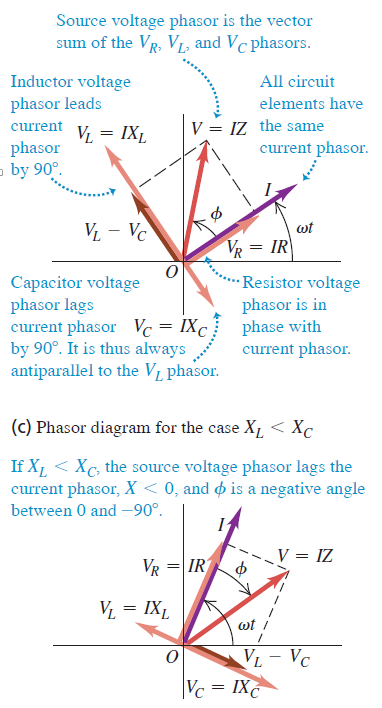
\includegraphics[width=2in]{images/Phasor diagram.png}
    \end{minipage}
};
%------------ Phasor header ---------------------
\node[fancytitle, right=10pt] at (box.north west) {Phasor Diagrams};
\end{tikzpicture}

%------------ AC Circuit Parallel ---------------
\begin{tikzpicture}
\node [mybox] (box){%
    \begin{minipage}{0.3\textwidth}
    Same voltages but currents are out of phase
    \vspace{.15cm}\\
    \textbf{Inductive and Capacitive Resistance}\\
    $X_L=\omega L$\\
    $X_C = \frac{1}{\omega C}$
    \vspace{.15cm}\\
    \textbf{Total Impedence Z: }\\
    $\left | \frac{1}{Z} \right |^2=\frac{1}{R^2}+(\frac{1}{X_L}-\frac{1}{X_C})^2$
    \vspace{.15cm}\\
    \textbf{Phase Angle:}\\
    $\tan\phi=R\cdot
    (\frac{1}{X_C}-\frac{1}{X_L})$\\
    arg$(i)-$arg$(v)=\phi$
    \vspace{.15cm}\\
    \textbf{Current as a function of time:}\\
    $I(t)=\frac{V_{max}}{Z}\cdot \sin(\omega t+ \phi_0+\phi)$\\
    *Note the angle is phi is added\\

    \end{minipage}
};
%------------ Ac Circuit Parallel ---------------------
\node[fancytitle, right=10pt] at (box.north west) {AC Parallel Current and Voltage};
\end{tikzpicture}

\medium

%------------ Electrostatics ---------------
\begin{tikzpicture}
\node [mybox] (box){%
    \begin{minipage}{0.3\textwidth}
    \textbf{Constants}
    \hline
    
    \vspace{.1cm}
    \begin{tabular}{lp{5cm} l}
        Electric Constant & $\varepsilon_\mathrm{0} = 8.854 \cdot 10^{-12} C^2/N\cdot m^{-2}$\\
        Coulomb's Constant & $\frac{1}{4 \pi\varepsilon_\mathrm{0} }=8.988\cdot 10^{9}  N\cdot m^2/C^2$\\
        Elementary Charge & $ e=1.60217662 \cdot 10^{-19}C$
		\vspace{.2cm}\\
		\end{tabular}
	
    \textbf{Laws}
    \hline
    
    
    \vspace{.1cm}
    \begin{tabular}{lp{4cm} l}
        Coulombs Law & $F=\frac{1}{4 \pi\varepsilon_\mathrm{0} }\cdot \frac{\left| q_1 q_2 \right |}{r^2}\hat{r}=q\vec{E}$\\
        Electric Field & $\vec{E}=\frac{\vec{F_0}}{q_0}=\frac{kq}{r^2}\hat{r}$
		\vspace{.2cm}\\
		\end{tabular}
	
	    \textbf{Charge Densities and Distributions}
    \hline
    
    
    \vspace{.1cm}
    \begin{tabular}{lp{4cm} l}
        Linear Charge Density & $\lambda = \frac{Q}{L}$\\
        Surface Charge density & $\sigma = \frac{Q}{A}$\\
        Charge Density & $\rho = \frac{Q}{V}$\\
        Non Uniform & $dQ=\lambda ds=\sigma dA = \rho dV$
		\end{tabular}
		
	\textbf{Electric Dipole}
	\hline
	\vspace{.1cm}
	\begin{tabular}{lp{4cm} l}
	    $\vec{p}=qd$\\
	    $\vec{\tau}=\vec{F}\cross\vec{d}$=pE\cdot\sin\varphi
	\end{tabular}
    \end{minipage}
};
%------------ Electrostatics Header ---------------------
\node[fancytitle, right=10pt] at (box.north west) {Electrostatics};
\end{tikzpicture}

%------------ Gauss Law ---------------
\begin{tikzpicture}
\node [mybox] (box){%
    \begin{minipage}{0.3\textwidth}
    \textbf{Flux Equations}
    \hline
    
    \vspace{.1cm}
    \begin{tabular}{lp{4cm} l}
        Gauss's Law & $\Phi_E = \oint \vec{E}\cdot d\vec{A} = \frac{Q_{encl}}{\varepsilon_\mathrm{0}}$\\
        Uniform E & $ \Phi_E = \vec{E}\cdot \vec{A} = EA\cdot \cos(\phi)$
		\vspace{.1cm}\\
		\end{tabular}
		
	\textbf{Electric Fields of Symmetric Objects}
	\hline
	\begin{tabular}{lp{4cm} l}
    Point Charge & $\vec{E}=k\frac{Q}{r^2}\hat{r}$\\
    Charged Rod & $\vec{E}=\frac{k\lambda l}{r\sqrt{r^2+\frac{l^2}{4}}}\hat{r}$\\
    Charged Ring & $\vec{E}=\frac{kQh}{(R^2+h^2)^{3/2}}\hat{n}$\\
    Charged Disk & $\vec{E}=2\pi k\sigma(\frac{1}{h}-\frac{1}{\sqrt{R^2+h^2}})\hat{n}$\\
    Infinite Plane & $\vec{E}=\frac{\sigma}{2\epsilon_{0}}\hat{n}$\\
    Infinite Wire & $\vec{E}=\frac{\lambda}{2 \pi r \epsilon_{0}}\hat{r}$\\
    Infinite Slab & $\vec{E}=\frac{\rho s}{2\epsilon_0}\hat{n}$ for $0\leq s\leq S$\\
    Infinite Cylinder & $\vec{E}=\frac{\rho r}{2\epsilon_0}\hat{r}$ for $0\leq r \leq R$\\
    Sphere Interior & $\vec{E}=\frac{\rho r}{3\epsilon_0}\hat{r}$ for $0\leq r \leq R$\\
    \end{tabular}
    Slabs at large distances emulate a plane\\
    Spheres at large distances emulate a point charge\\
    Cylinders at large distances emulate a wire
    \end{minipage}
};
%------------ Gauss Law Header ---------------------
\node[fancytitle, right=10pt] at (box.north west) {Gauss's Law};
\end{tikzpicture}


\end{multicols*}


%------------ CC License -----------------------------
\doclicenseThis

\linespread{1.3}

\begin{multicols*}{3}
\tikzstyle{mybox} = [draw=black, fill=white, very thick,
    rectangle, rounded corners, inner sep=10pt, inner ysep=10pt]
\tikzstyle{fancytitle} =[fill=black, text=white, font=\bfseries]


%--------------New Pages for Electrical --------------------
\newpage
\medium
%--------------New Pages for Electrical --------------------

%------------ Electric Potential ---------------
\begin{tikzpicture}
\node [mybox] (box){%
    \begin{minipage}{0.3\textwidth}
    Generally for Work:\\
    $W_{a \rightarrow b} = U_a - U_b = -\Delta U$\\
    $U=0$ is at infinite charge separation 
    
    \textbf{Point Charges}
    \hline
    
    \vspace{.1cm}
    \begin{tabular}{lp{5cm} l}
        Two charges & $U = \frac{1}{4 \pi \varepsilon_\mathrm{0}}\cdot \frac{qq_0}{r}$\\
        Multiple Charges & $U = \frac{q_0}{4 \pi \varepsilon_\mathrm{0}}\cdot (\frac{q_1}{r_1}+\frac{q_2}{r_2}+...\frac{q_n}{r_n})$\\
        Sum of system & $U_{net} =  \frac{1}{4 \pi \varepsilon_\mathrm{0}}\cdot \sum_{i<j}\frac{q_i q_j}{r_{ij}} $

		\vspace{.1cm}
		\end{tabular}
	
	\\
    \textbf{Voltage and Potential}
    \hline


    \medium
    {
    \vspace{.1cm}
    Generally, $V(\infty)=0$ when not specified\\
    Difference Notation is $V_{ab}=V_a-V_b$\\
    Means $V_a$ with respect to $V_b$\\
    \begin{tabular}{lp{4cm} l}
        Voltage &    $\frac{W_{a \rightarrow b}}{q_0}=-\frac{\Delta U}{q_0}=V_a-V_b$\\
        Point Charge & $V = \frac{1}{4 \pi \varepsilon_\mathrm{0}}\cdot \frac{q}{r}$\\
        Multiple Charges & $V = \frac{1}{4 \pi \varepsilon_\mathrm{0}}\cdot (\frac{q_1}{r_1}+\frac{q_2}{r_2}+...\frac{q_n}{r_n})$\\
        Distributed Charge & $V =  \frac{1}{4 \pi \varepsilon_\mathrm{0}}\cdot \int \frac{dq}{r} $\\
        \\
        \textbf{V function of E} & $-\frac{\Delta U}{q_0} = V_a - V_b =  \int_{a}^{b} \vec{E}\cdot \vec{dl} $\\
        Infinitesimals & $dV=-\vec{E} \cdot \vec {dl} $\\
        \textbf{E function of V} &
        $\vec{E}=\vec{\nabla}V$\\
        Expanded & $\vec{E}=\frac{\partial V}{\partial x}\hat{i}+\frac{\partial V}{\partial y}\hat{j}+\frac{\partial V}{\partial z}\hat{k}$\\
        Radial & $\vec{E}=\frac{dV}{dr}$
		\end{tabular}
	}

    
    \end{minipage}
};
%------------ Electric Potential Header ---------------------
\node[fancytitle, right=10pt] at (box.north west) {Electric Potential};
\end{tikzpicture}

%------------ Dielectrics  ---------------
\begin{tikzpicture}
\node [mybox] (box){%
    \begin{minipage}{0.3\textwidth}
        \textbf{Capacitance and Energy}
    \hline
    
    \vspace{.1cm}
    Parallel Plates: $ C = \frac{Q}{V_{ab}}=\epsilon_\mathrm{0} \frac{A}{d}$\\
     Energy density: $u=\frac{1}{2}\epsilon_\mathrm{0}E^2$ and $U = \int u \cdot dV$\\
     Stored Energy & $U=\frac{Q^2}{2C}=\frac{1}{2}CV^2=\frac{1}{2}QV$\\
    \textbf{Dielectrics}
    \hline
   \begin{tabular}{lp{4cm} l}
        Dielectric Constant & $\kappa = \frac{C}{C_0}$\\
        V for constant Q & $V = \frac{V_0}{\kappa}$\\
        E for constant Q & $E = \frac{E_0}{\kappa}$\\
        Induced Charge & $\sigma_i=\sigma(1-\frac{1}{\kappa})$\\
        Dielectric Gauss & $\oint \kappa\vec{E}\cdot \vec{dA} = \frac{Q_{conductor}}{\varepsilon_\mathrm{0}}$\\
       
         
        
		\end{tabular}

    \end{minipage}
};
%------------ Dielectrics Header ---------------------
\node[fancytitle, right=10pt] at (box.north west) {Capacitance and Dielectrics};
\end{tikzpicture}

\medium
%------------ Magnetism  ---------------
\begin{tikzpicture}
\node [mybox] (box){%
    \begin{minipage}{0.3\textwidth}
    \textbf{Cross Product}
    \hline\\
    \vspace{.1cm}
    Use right hand rule for direction\\
    $\vec{v} \times \vec{B} = vB\cdot sin(\phi)$
    \vspace{.1cm}

    \textbf{Magnetic Force}
    \hline
   \begin{tabular}{lp{4cm} l}
   Magnetic Force & $\vec{F} = q \vec{v} \times \vec{B}$\\
   \textbf {Lorentz Force Equation} & \\  
   Net Elec \& Magnetic F & $\vec{F} = q (\vec{E} + \vec{v} \times \vec{B})$
     \vspace{.1cm}
		\end{tabular}
		
		
	    \textbf{Magnetic Flux and Gauss}
    \hline
   \begin{tabular}{lp{4cm} l}
   Magnetic Flux& $\Phi_B=\int\vec{B}\cdot d\vec{A}$ \\
   & \hspace{13} $ = \int B * cos(\phi)dA$\\
   \textbf {Gauss Law} & $\oiint \vec{B}\cdot d\vec{A} = 0$\\
   		\end{tabular}
   		
   	\textbf{Cyclotron Motion}
    \hline
   \begin{tabular}{lp{4cm} l}
    Force from field & $F = qv_{\perp}B=\frac{mv_{\perp}^2}{R}$ \\
    Radius & $R=\frac{mv_{\perp}}{qB}$\\
    Frequency & $\omega = \frac{v_{\perp}}{R}=\frac{qB}{m}$\\
    
   	\end{tabular}

    \end{minipage}
};
%------------ Magnetism Header ---------------------
\node[fancytitle, right=10pt] at (box.north west) {Magnetism};
\end{tikzpicture}

%------------ Current and Motors  ---------------
\begin{tikzpicture}
\node [mybox] (box){%
    \begin{minipage}{0.3\textwidth}
    \begin{center}
    \framebox{
    \parbox[t][.4cm]{3cm}{
     $\mu_0=4\pi\cdot 10^{-7}N/A^2$\\
    } 
}
\end{center}
    \textbf{Current through wire}
    \hline\\
    
    \begin{tabular}{lp{4cm} l}
    Straight Wire  & $\vec{F}=I\cdot \vec{l} \times \vec{B}$\\
    Wire segment & $ d\vec{F} = I d\vec{l} \times \vec{B}$\\
    Mag Field Produced & $B=\frac{\mu_0I}{2\pi r} $\\
    Two Wires Attraction & $\frac{F}{L}=\frac{\mu_0 I_1 I_2}{2\pi r}$\\
    \end{tabular}
    \textbf{Dipole and Torque}
    \hline
    \begin{tabular}{lp{4cm} l}
    Dipole Moment & $\vec{\mu}=NI\vec{A}$\\
    Wire Loop Torque & $\tau = \mu B$ sin$(\phi) $\\
    Torque Vector & $\vec{\tau} =\vec{\mu} \times \vec{B}$\\
    Dipole Potential & $U=-\vec{\mu} \cdot \vec{B} = - \mu B$ cos$\phi $
   	\end{tabular}
   	\begin{center}
       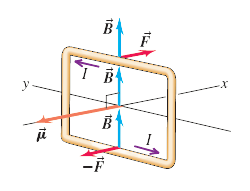
\includegraphics[width=1.4in]{images/Wire Loop.png} 
    \end{center}
   	

    \end{minipage}
};
%------------ Currents Magnets Header---------------------
\node[fancytitle, right=10pt] at (box.north west) {Current Motors Magnets};
\end{tikzpicture}

%------------ Maxwell  ---------------
\begin{tikzpicture}
\node [mybox] (box){%
    \begin{minipage}{0.3\textwidth}
    \begin{tabular}{lp{4cm} l}
    $\mu_0\epsilon_0=\frac{1}{c^2}$
    \end{tabular}
    \\
    \textbf{Integral Form}
    \hline\\
    \vspace{.1cm}
    \begin{tabular}{lp{4cm} l}
    $\oiint\vec{E}\cdot d\vec{A}=\frac{q_{enc}}{\epsilon_0}$\\
    $\oiint\vec{B}\cdot d\vec{A}=0$\\
    $\oint\vec{E}\cdot d\vec{s}=-\frac{\Phi_B}{dt}$\\
    $\oint\vec{B}\cdot d\vec{s}=\mu_0I_{enc}+\epsilon_0\mu_0\frac{d\Phi_E}{dt}$
    \end{tabular}
    \vspace{.1cm}

    \textbf{Differential Form}
    \hline
    \begin{tabular}{lp{4cm} l}
    $\vec{\nabla}\cdot\vec{E}=\frac{\rho}{\epsilon_0}$\\
    $\vec{\nabla}\cdot\vec{B}=0$\\
    $\vec{\nabla}\times\vec{E}=-\frac{\partial\vec{B}}{\partial t}$\\
    $\vec{\nabla}\times\vec{B}=\mu_0\vec{J}+\mu_0\epsilon_0\frac{\partial\vec{E}}{\partial t}$
	\end{tabular}
    \vspace{.1cm}

    \textbf{Multivariable Calculus Formulas}
    \hline
    \begin{tabular}{lp{4cm} l}
    Stokes Theorem & $\iint\vec{\nabla}\times\vec{v}\cdot dA=\oint\vec{v}\cdot d\vec{l}$\\
    Divergence Theorem & $\iiint\vec{\nabla}\cdot\vec{v}d^3r=\oiint\vec{v}\cdot d\vec{A}$
	\end{tabular}

    \end{minipage}
};
%------------ Maxwell's Equations ---------------------
\node[fancytitle, right=10pt] at (box.north west) {Maxwell's Equations};
\end{tikzpicture}


%------------ Magnetic Fields ---------------
\begin{tikzpicture}
\node [mybox] (box){%
    \begin{minipage}{0.3\textwidth}
    \textbf{Magnetic Field Equations}
    \hline\\
    
    \begin{tabular}{lp{5cm} l}
    Biot-Savart Law  & $d\vec{B}=\frac{\mu_0}{4\pi}\frac{I\cdot d\vec{l}\times \hat{r}}{r^2}$\\
    Ampere's Law & $\oint \vec{B}\cdot d\vec{l} =\mu_0 I_{encl}$\\
    Moving Particle  & $\vec{B}=\frac{\mu_0}{4\pi}\frac{q\vec{v}\times \hat{r}}{r^2}$\\
    Loop of Current & $\vec{B}=\frac{\mu_0IR^2}{2(h^2+R^2)^{3/2}}\hat{n}$\\
    Straight Wire & $B=\frac{\mu_0I}{4\pi r}\sin\theta|^{\theta_R}_{\theta_L}=\frac{\mu_0Ix}{4\pi r\sqrt{x^2+r^2}}|^{x_R}_{x_L}$\\
    Straight Wire & $B=\frac{\mu_0Il}{4\pi r\sqrt{r^2+\frac{l^2}{4}}}$ at center only\\
    Infinite Wire & $B=\frac{\mu_0I}{2\pi r}$ for $l \gg r$
    \end{tabular}
     \textbf{Solenoids}
    \hline
    \vspace{.1cm}
        \begin{tabular}{lp{5cm} l}
        Coil Density & $n = N/L$\\
        Toroid & $B=\frac{\mu_0IN}{2\pi r}$\\
        Infinite Solenoid & $B=\mu_0In$\\
        Finite Solenoid & $B=\frac{\mu_0Inx}{2\sqrt{x^2+R^2}}|^{x_R}_{x_L}$\\
        & $B=\frac{\mu_0}{2}I\cdot n(\cos\theta_R - \cos\theta_L)$\\
    
    \end{tabular}

       	\begin{center}
       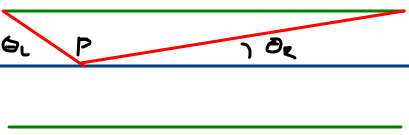
\includegraphics[width=1.4in]{images/solenoid.png} 
    \end{center}
    
    \end{minipage}
};
%------------ Magnetic Fields Header ---------------------
\node[fancytitle, right=10pt] at (box.north west) {Magnetic Fields};
\end{tikzpicture}

%------------ Electromagnetic Induction ---------------
\begin{tikzpicture}
\node [mybox] (box){%
    \begin{minipage}{0.3\textwidth}

    \textbf{Faradays's Law}
    \hline
    \vspace{.1cm}
        \begin{tabular}{lp{4cm} l}
    Induced Emf  &  $\mathcal{E} =\oint \vec{E}\cdot \vec{dl}  = -\frac{d\Phi_B}{dt}$\\
    Solenoid Emf & $\mathcal{E} = -\frac{d\Phi_B}{dt} = -\mu_0 n A \frac{dI}{dt}$\\
    Motional Emf & $\mathcal{E} =\oint (\vec{v}\times \vec{B})\cdot d\vec{l}$\\
    For moving Bar & $\mathcal{E} = vBL$
    \end{tabular}
    
    \begin{center}
    \framebox{
    \parbox[t][1.5cm]{7.5cm}{
    \small
         The direction of any magnetic induction effect is such as to oppose the cause of the effect.  Induced current direction in a loop opposes the change in flux.
    } 
}
\small
\end{center}
    \textbf{Ampere-Maxwell Law}
    \hline
    \vspace{.1cm}
        \begin{tabular}{lp{5cm} l}
    Displacement Current & $i_{disp}=\epsilon_0\frac{d\Psi_E}{dt}$\\
    Ampere-Maxwell Law & $\oint\vec{B}\cdot d\vec{s}=\mu_0I_{enc}+\epsilon_0\mu_0\frac{d\Phi_E}{dt}$
    \end{tabular}
    
    \textbf{Electromagnetic Waves (not on final)}
    \hline
    \vspace{.1cm}
        \begin{tabular}{lp{5cm} l}
        Proportionality & $E=cB$\\
        Speed of Light & $\mu_0\epsilon_0=\frac{1}{c^2}$\\
        Solar Wind & $\vec{S}=\frac{\vec{E}\times\vec{B}}{\mu_0}$\\
        Intensity & $S_{avg}=I=\frac{E_{max}B_{max}}{2\mu_0}$\\
        Radiation Pressure & $P_{rad}=\frac{I}{c}=\frac{S_{avg}}{c}$
    \end{tabular}

    \end{minipage}
};
%------------ Electromagnetic Induction Header ---------------------
\node[fancytitle, right=10pt] at (box.north west) {Electromagnetic Induction};
\end{tikzpicture}






\end{multicols*}




\end{document}


Contact GitHub API Training Shop Blog About
© 2016 GitHub, Inc. Terms Privacy Security Status Help